\documentclass[t,12pt]{beamer}
\usepackage[utf8]{inputenc}
\usepackage[T1]{fontenc}
\usepackage{fancyhdr} % pour personnaliser les en-têtes
\usepackage{lastpage}
\usepackage[frenchb]{babel}
\usepackage{amsfonts,amssymb}
\usepackage{amsmath,amsthm}
\usepackage{paralist}
\usepackage{enumerate}
\usepackage{xspace}
\usepackage{xcolor}
\usepackage{variations}
\usepackage{xypic}
\usepackage{eurosym,multicol}
\usepackage{graphicx}
\usepackage[np]{numprint}
\usepackage{hyperref} 
\usepackage{setspace}
\usepackage{listings} % pour écrire des codes avec coloration syntaxique  

\usepackage{tikz}
\usetikzlibrary{calc, arrows, plotmarks,decorations.pathreplacing}
\usepackage{colortbl}
\usepackage{multirow}


\newtheorem{defi}{Définition}
\newtheorem{thm}{Théorème}
\newtheorem{thm-def}{Théorème/Définition}
\newtheorem{rmq}{Remarque}
\newtheorem{prop}{Propriété}
\newtheorem{cor}{Corollaire}
\newtheorem{lem}{Lemme}
\newtheorem{ex}{Exemple}
\newtheorem{cex}{Contre-exemple}
\newtheorem{prop-def}{Propriété-définition}
\newtheorem{exer}{Exercice}
\newtheorem{nota}{Notation}
\newtheorem{ax}{Axiome}
\newtheorem{appl}{Application}
\newtheorem{csq}{Conséquence}
%\def\di{\displaystyle}


\newcommand{\vtab}{\rule[-0.4em]{0pt}{1.2em}}
\newcommand{\V}{\overrightarrow}
\renewcommand{\thesection}{\Roman{section} }
\renewcommand{\thesubsection}{\arabic{subsection} }
\renewcommand{\thesubsubsection}{\alph{subsubsection} }
\newcommand{\C}{\mathbb{C}}
\newcommand{\R}{\mathbb{R}}
\newcommand{\Q}{\mathbb{Q}}
\newcommand{\Z}{\mathbb{Z}}
\newcommand{\N}{\mathbb{N}}



\usetheme{Warsaw}

\title{Questions sur les probabilités }
\author{}
\date{}
\begin{document}
\maketitle	

\begin{frame}
	\frametitle{Question 1: }
	Une urne contient 3 boules bleues, 5 boules rouges et 12 boules noires. On tire au hasard une boule. 
	
	\begin{enumerate}
		\item Donner l'univers associé à cette expérience.  
		\item Pour les évènements ci-dessous, exprimer les évènements contraires:
		\begin{enumerate}[$\square$]
			\item $A : \{"\text{La boule tirée est bleue}"\}$
			\item $B : \{"\text{La boule tirée n'est pas noire}"\}$
			\item $C : \{"\text{La boule tirée est jaune}"\}$
		\end{enumerate}
	\hfill\\
		\item Donner la valeur des probabilités suivantes :\\ 
		\begin{multicols}{3}
			\begin{enumerate}[$\square$]
				\item $P(\overline{A})$
				\item $P(\overline{B})$
				\item $P(\overline{C})$
			\end{enumerate}
		\end{multicols}
	
	\end{enumerate}
	

\end{frame}

\begin{frame}
	\frametitle{Question 2: Lancer trois dés et faire la somme}
	Voici un programme Python, 
	\begin{figure}
		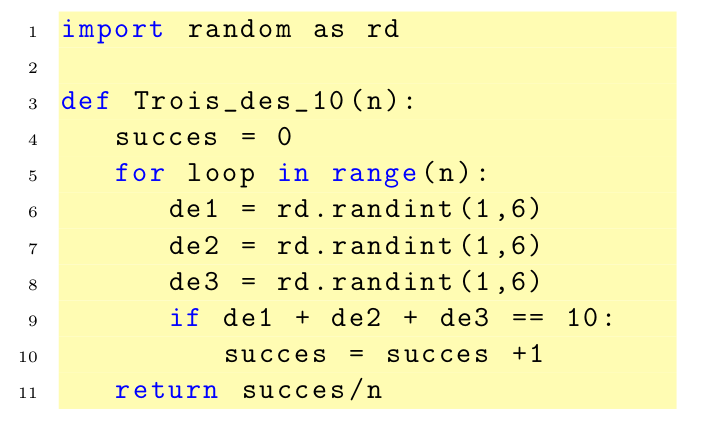
\includegraphics[scale=0.3]{1.png}
	\end{figure}\hfill\\[-0.4cm]
	\begin{enumerate}
		\item Recopier ce programme Python en respectant la syntaxe. 
		\item Faites une phrase qui explique ce qu'exécute la fonction Trois\_des\_10 lorsqu'on lui donne un entier naturel $n$.	
	\end{enumerate}
\end{frame}
	
\begin{frame}
	\frametitle{Question 3: }
	
	Lors d'une compétition sportive en région parisienne, la répartition des participants et des participantes est la suivante:
	\begin{center}
		\begin{tabular}{|l|c|c|}
			\cline{2-3}
			\multicolumn{1}{c|}{} & Hommes & Femmes \\
			\hline
			Bagneux  &  29 &  51\\ \hline
			Montrouge & 16 & 34\\
			\hline 
		\end{tabular}
	\end{center}
	On choisit au hasard une personne de ce groupe. 	
	\begin{enumerate}
		\item Donner le nombre de participants à cette compétition.
		\item Donner la probabilité des évènements suivants :
		\begin{enumerate}[$\square$]
			\item $A:\{"\text{La personne est une femme}"\}$ 
			\item $B:\{"\text{La personne habite à Bagneux}"\}$ 
			\item $C:\{"\text{La personne  habite à Montrouge et est un homme}"\}$
			\item $D:\{"\text{Être une femme ou habiter à Bagneux }"\}$  	
		\end{enumerate}
	\end{enumerate}	
\end{frame}

\begin{frame}
	\frametitle{Question 4: }
			Une urne contient 12 boules blanches et 8 boules noires. On tire au hasard une boule.
	\begin{enumerate}
		\item Quelle est la probabilité de tirer une boule blanche?
		\item Recopier et compléter le programme Python ci-dessous afin qu'il modélise cette expérience aléatoire. 
		\begin{figure}
			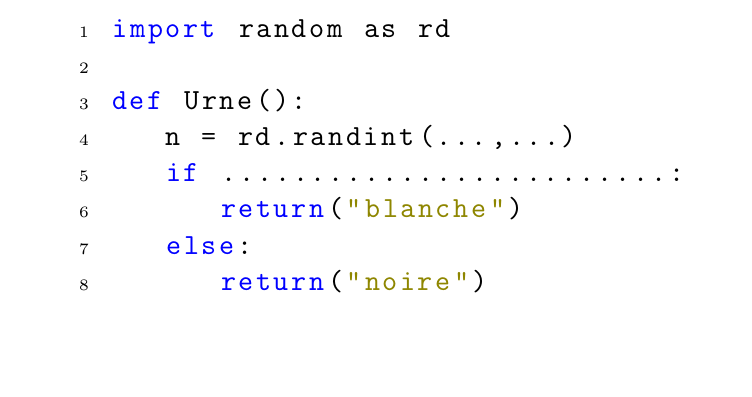
\includegraphics[scale=0.4]{2.png}
		\end{figure}\hfill\\
	\end{enumerate}
\end{frame}


\begin{frame}
	\frametitle{Question 5: }
	On place dans une boite des jetons rouges, verts et bleus qui sont numérotés par le chiffre 1 et le chiffre 2. On tire au hasard un jeton et on note sa couleur et son numéro. Voici le tableau des probabilités associées aux issues de cette expérience aléatoire. 
	
	\begin{center}
		\begin{tabular}{|l|c|c|c|}
			\cline{2-4}
			\multicolumn{1}{c|}{} & Rouge & Vert & Bleu  \\
			\hline
			1  &  0,1 &  0,3& 0\\ \hline
			2 & 0,3 & 0,1& 0,2\\
			\hline 
		\end{tabular}
	\end{center} 
	\begin{enumerate}
		\item Quelle est la probabilité qu'il soit rouge?
		\item Quelle est la probabilité qu'il porte le numéro 2?
		\item Quelle est la probabilité qu'il soit bleu et qu'il porte le numéro 1 ? 
		\item Quelle est la probabilité qu'il soit vert ou qu'il porte le numéro 1 ?
	\end{enumerate}
\end{frame}

\begin{frame}
	\frametitle{Question 6: }
	Ce programme Python modélise le lancer d'une pièce truquée qui a tendance à donner plus de "Face" que de "Pile". 
	\begin{figure}
		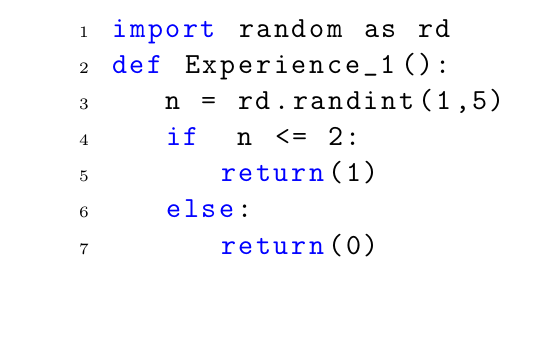
\includegraphics[scale=0.4]{3.png}
	\end{figure}\hfill\\[-1.5cm]
\begin{enumerate}
	\item À quelle issue est associée le nombre 1 dans ce programme et à quelle issue est associée le nombre 0 dans ce programme? 
	\item Quelle est la probabilité de l'évènement $P: \{"\text{Avoir un pile}"\}$ et en déduire la probabilité de $\overline{P}$?
	%\item Changer ce programme Python pour qu'il modélise le lancé d'une pièce truquée qui a $6$ fois plus de chance de faire "Pile" que "Face".  
\end{enumerate}
\end{frame}
\end{document}